\documentclass{amsart}

\usepackage{graphicx, fancyhdr, rotating, float} % see geometry.pdf on how to lay out the page. There's lots.
\usepackage[a4paper, margin=0.5in, includeheadfoot, headheight=2cm, footskip=2cm]{geometry}
\usepackage{booktabs}
\usepackage{multirow}


\usepackage{color}
\usepackage{xcolor}
\usepackage{listings}
\usepackage{numprint}
\npthousandsep{,}
\npdecimalsign{.}

\usepackage{caption}
\DeclareCaptionFont{white}{\color{white}}
\DeclareCaptionFormat{listing}{\colorbox{gray}{\parbox{\textwidth}{#1#2#3}}}
\captionsetup[lstlisting]{format=listing,labelfont=white,textfont=white}



% See the ``Article customise'' template for come common customisations
\providecommand{\e}[1]{\ensuremath{\times 10^{#1}}}
%\setlength{\headheight}{2cm}

\graphicspath{{./images/}} % Specify images directory


% Title and document details
\newcommand{\titleinfo}{$job.title} 
\title{\titleinfo}
\pagestyle{fancy}
\fancyhf{}
\lhead{}
\chead{
\includegraphics[height=2.5cm]{header.png}}
\renewcommand{\headrulewidth}{0pt}
\rhead{}
\rfoot{\thepage}
\lfoot{\titleinfo}
\author{$job.author}
\date{\today}

%%% BEGIN DOCUMENT
\begin{document}

% First page (title and toc)
\maketitle
\thispagestyle{fancy}
\tableofcontents


% General spacing for the document to use after the title and toc
\linespread{1.2} % A little more line spacing than usual
\setlength\parindent{0pt} % Removes indentation from paragraphs
\setlength{\parskip}{0.25cm} % Adds an extra bit of linespacing between paragraphs
\setlength{\belowbottomsep}{2ex} % Ensure a decent gap before the footer



\newpage
\section{General Information}
\begin{description}
\item[Project title] \titleinfo
\item[Name of collaborator] $job.collaborator
\item[Staff member] $job.author
\item[SEQINFO ticket] $job.jiraSeqinfoId
\item[MISO ticket] $job.misoId
\item[Date at job completion] \today
\end{description}


\section{Software Used}

This report was automatically generated by RAMPART (Robust Automatic MultiPle AssembleR Toolkit).  RAMPART is a TGAC project that builds first pass assemblies from sequenced reads by chaining together a number of 3rd party tools.  The main tools used for this job are specified in Table \ref{tab:software-used}.

\begin{table}[h]
\begin{tabular}{lll}
\toprule
Task & Tool & Version \\ \midrule
Quality Trimming & $settings.qtTool & $settings.qtToolVersion \\
Contig Assembly & $settings.massTool & $settings.massToolVersion \\
Scaffolding & $settings.impScfTool & $settings.impScfToolVersion \\
Gap Closing & $settings.impDegapTool & $settings.impDegapToolVersion \\
\bottomrule
\end{tabular}
\caption{Software used for this RAMPART job.}
\label{tab:software-used}
\end{table}

\pagebreak
\newpage
\section{Input Libraries}

The job requested the raw sequenced libraries specified in Table \ref{tab:libraries}.  

\begin{table}[h]
\begin{tabular}{lrrll}
\toprule
Library Name & Max Read Length & Avg Insert Size & Usage & Orientation \\ \midrule
#foreach($lib in $job.libsRaw)ls
$lib.name & $lib.readLength & $lib.averageInsertSize & $lib.usage.toString() & $lib.seqOrientation \\
#end
\bottomrule
\end{tabular}
\caption{Libraries used for this RAMPART job.}
\label{tab:libraries}
\end{table}

\pagebreak
\newpage
\section{Description of the Complete Workflow}

Figure \ref{fig:workflow} represents the general workflow applied to the raw reads produced from the sequencing device.  Initially, the raw dataset is quality trimmed to produce a second input dataset.  Then each dataset is processed through an assembler using multiple k-mer values producing multiple assemblies.  These assemblies are analysed and the best assembly is selected to be enhanced using scaffolding and gap closing tools.  Optionally, scaffold deduplication and clipping can be applied to further enhance the assembly.

\begin{figure}[H]
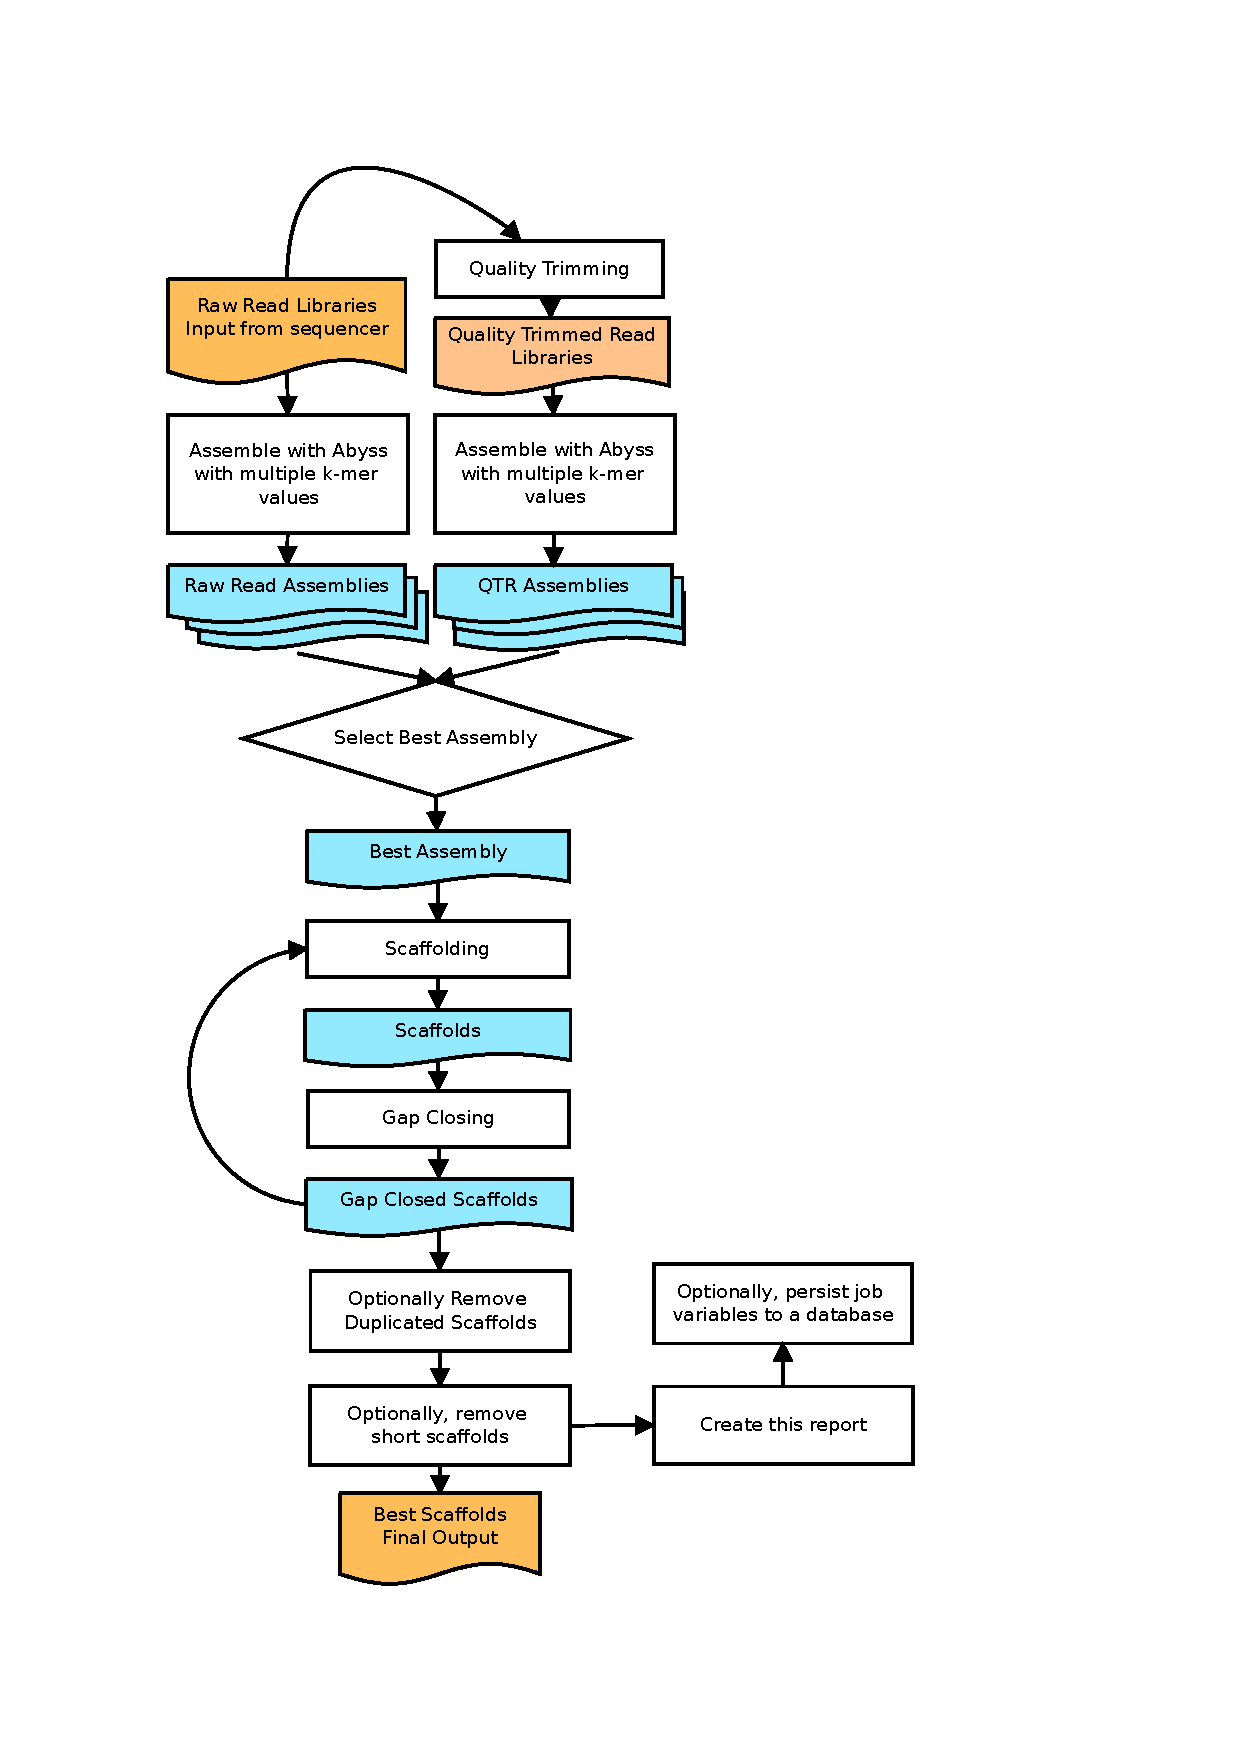
\includegraphics[width=13cm]{Workflow.pdf}
\caption{Typical First Pass Assembly Workflow}
\label{fig:workflow}
\end{figure}


\pagebreak
\newpage
\section{Quality Trimming}

The reads in the libraries mentioned in Table \ref{tab:libraries} were analysed based on the sequence quality scores, and those sequences which dipped below a certain threshold were either trimmed or excluded.  The tool: $settings.qtTool was used to do this.  This tool was configured so that the 3' ends of reads are trimmed where quality degrades beyond a threshold score of Q-$settings.qtThreshold.  Any trimmed reads must still exceed $settings.qtMinLen base pairs in length otherwise the whole read is discarded.  The statistics for the RAW and Quality Trimmed (WT) datasets are shown in Table \ref{tab:dataset-stats}.

\begin{table}[h]
\begin{tabular}{lllrrrr}
\toprule
Library & Dataset & File & \# Reads & \%GC & Total Bases & Est. Coverage  \\ \midrule
#foreach($lib in $job.libsRaw)
$lib.name & $lib.dataset & PE1 & \numprint{$lib.filePaired1.seqCount} & \nprounddigits{2} $\numprint{$lib.filePaired1.gCContent}$ \npnoround & \numprint{$lib.filePaired1.baseCount} & $0 \times$ \\ 
$lib.name & $lib.dataset & PE2 & \numprint{$lib.filePaired2.seqCount} & \nprounddigits{2} $\numprint{$lib.filePaired2.gCContent}$ \npnoround & \numprint{$lib.filePaired2.baseCount} & $0 \times$ \\
#if( $lib.seFile )
$lib.name & $lib.dataset & SE & \numprint{$lib.seFile.seqCount} & \nprounddigits{2} $\numprint{$lib.seFile.gCContent}$ \npnoround & \numprint{$lib.seFile.baseCount} & $ xxx \times$ \\
#end
#end
#foreach($lib in $job.libsQt)
$lib.name & $lib.dataset & PE1 & \numprint{$lib.filePaired1.seqCount} & \nprounddigits{2} $\numprint{$lib.filePaired1.gCContent}$ \npnoround & \numprint{$lib.filePaired1.baseCount} & $0 \times$ \\ 
$lib.name & $lib.dataset & PE2 & \numprint{$lib.filePaired2.seqCount} & \nprounddigits{2} $\numprint{$lib.filePaired2.gCContent}$ \npnoround & \numprint{$lib.filePaired2.baseCount} & $0 \times$ \\
#if( $lib.seFile )
$lib.name & $lib.dataset & SE & \numprint{$lib.seFile.seqCount} & \nprounddigits{2} $\numprint{$lib.seFile.gCContent}$ \npnoround & \numprint{$lib.seFile.baseCount} & $ xxx \times$ \\
#end
#end
\bottomrule
\end{tabular}
\caption{Basic Statistics for each library before and after quality trimming (Dataset `RAW' indicates before quality trimming and `QT' indicates after quality trimming.  #if($job.estGenomeSize) Estimated Coverage assumes even distribution of reads against a genome size of $job.estGenomeSizeMb.#end}
\label{tab:dataset-stats}
\end{table}



\newpage
\section{Multiple Contig Assemblies}

The datasets we assembled the reads by $settings.massTool $settings.massToolVersion using a variety of k-mer lengths.  Various contig size metrics were gathered from each contig assembly in order to determine the optimal k-mer setting from which to build the final scaffolded assembly.  Graphs generated from some of the key size metrics across all k-mer values are shown in Table \ref{fig:contig_assembly_graphs}.

\begin{table}[H]
\begin{center}
\begin{tabular}{c|c|c}
\includegraphics[height=5cm]{Mass_NBC.pdf} & \includegraphics[height=5cm]{Mass_TB.pdf} & \includegraphics[height=5cm]{Mass_N.pdf}\\ \midrule 
\includegraphics[height=5cm]{Mass_AL.pdf} & \includegraphics[height=5cm]{Mass_ML.pdf} & \includegraphics[height=5cm]{Mass_N50.pdf} 
\end{tabular}
\end{center}
\caption{Plots showing various assembly size metrics against kmer value. Black lines represent the Raw Dataset.  Red lines the quality trimmed dataset.}
\label{fig:contig_assembly_graphs}
\end{table}

RAMPART normalises and weights contig assembly statistics in order to generate an overall assembly quality score.  The weightings related to each size metric are shown in Table \ref{tab:weightings}.  The overall contig assembly scores are shown in Figure \ref{fig:contig_assembly_scores}.  The contig assembly that scores the maximum value has a k-mer value of $best_mass_asm.kmer and it was from the $best_mass_asm.dataset dataset.

\begin{table}[H]
\begin{center}
\begin{tabular}{lr}
\toprule
Metric & Weighting \\ \midrule
\# contigs & $weightings.nbContigs \\
N\% & $weightings.nPerc \\
Max Length & $weightings.maxLen \\
Avg Length & $weightings.avgLen \\
N50 & $weightings.n50 \\
\bottomrule
\end{tabular}
\end{center}
\caption{Weightings applied to each assembly size metric.}
\label{tab:weightings}
\end{table}


\begin{figure}[H]
\includegraphics[width=13cm]{Mass_Scores.pdf}
\caption{Overall contig assembly scores.  A score is the result of summing the normalised and weighted metrics as shown in Table \ref{tab:weightings}.  The black line represents score for the RAW dataset.  The red line represents scores for the QT dataset.  Both datasets are plotted against the kmer value used for the assembly.}
\label{fig:contig_assembly_scores}
\end{figure}




\newpage
\section{Assembly Enhancement}

The best contig assembly was then enhanced through a series of processes shown in Table \ref{tab:enhancingSteps}

\begin{table}[H]
\begin{center}
\begin{tabular}{clll}
\toprule
Index & Stage Type & Tool & Tool Version \\ \midrule
1 & SCAFFOLDING & SCF TOOL & 1.0 \\
\bottomrule
\end{tabular}
\end{center}
\caption{Processes applied in series in the assembly enhancement stage.}
\label{tab:enhancingSteps}
\end{table}


The tool: $settings.impScfTool $settings.impScfToolVersion was used for scaffolding.  The tool: $settings.impDegapTool $settings.impDegapToolVersion was used for the gap closing. The results of this step are shown in the Figure \ref{fig:scaffold_assembly_graphs}.


\begin{table}[H]
\begin{center}
\begin{tabular}{c|c|c}
\includegraphics[height=5cm]{Improver_NBC.pdf} & \includegraphics[height=5cm]{Improver_TB.pdf} & \includegraphics[height=5cm]{Improver_N.pdf}\\ \midrule 
\includegraphics[height=5cm]{Improver_AL.pdf} & \includegraphics[height=5cm]{Improver_ML.pdf} & \includegraphics[height=5cm]{Improver_N50.pdf} 
\end{tabular}
\end{center}
\caption{Plots showing various assembly size metrics against enhancement stage.}
\label{fig:scaffold_assembly_graphs}
\end{table}

The final assembly has $final_asm.nbContigs scaffolds, and contains $final_asm.nbBases bases.  The average scaffold length is \nprounddigits{0}$\numprint{$final_asm.avgLen}$ \npnoround and the maximum scaffold length is $final_asm.maxLen.  Finally, the N50 score is $final_asm.n50.


\newpage
\section{Validation}

No validation on the final assembly is done at present.  However, we expect to be able to tell you about many more assembly quality metrics in the future.


\newpage
\section{Accessing the Data}

The RAMPART job directory is located at:

\begin{lstlisting}[label=path:1]
$locations.getJobDir()
\end{lstlisting}

The original reads, as well as the quality trimmed reads can be found at the following location:

\begin{lstlisting}[label=path:1]
$locations.getReadsDir()
\end{lstlisting}

\emph{Note}: The quality trimmed read files referred to in this report can be identified with the *.qt.* tag.

The Abyss assemblies and statistics for each dataset can be found at the following location:

\begin{lstlisting}[label=path:1]
$locations.getMassDir()
\end{lstlisting}


The assemblies, statistics and other data for the assembly improvement stage can be found at the following location:

\begin{lstlisting}[label=path:1]
$locations.getImproverDir()
\end{lstlisting} 


The final assembly can be found at the following location:

\begin{lstlisting}[label=path:1]
$final_asm.getFilePath()
\end{lstlisting}


\end{document}

